\section{Obiettivi di qualità} 
\subsection{Qualità di processo}

Al fine di garantire la qualità del prodotto in ogni fase di realizzazione, si deve garantire la qualità dei Processi\ped{g} che lo definiscono; per questo motivo si è deciso di utilizzare lo standard ISO/IEC 15504 denominato SPICE\ped{g}, che rende disponibili strumenti adatti a valutarli.

Per applicare correttamente questo modello si deve utilizzare il ciclo di Deming (ciclo PDCA) il quale definisce una metodologia di controllo dei Processi\ped{g} durante il loro ciclo di vita\ped{g} che consente di migliorarne in modo continuativo la qualità.

Tutti i Processi\ped{g} dovranno quindi essere sottoposti a valutazione in modo da verificarne la qualità ed eventualmente facilitarne il miglioramento. A tale scopo lo SPICE\ped{g} definisce nove attributi di Processo\ped{g} per effettuare una migliore valutazione:
\begin{enumerate}
\item \textbf{Process performance}\\
Gli indicatori della performance di Processo\ped{g} sono:
\begin{itemize} 
\item I lavori identificati come input al Processo\ped{g} (input work products);
\item I lavori identificati come output del Processo\ped{g} (output work products);
\item Le azioni compiute per trasformare gli input work products in output work products.
\end{itemize}

\item \textbf{Performance Management}\\
L’attuazione di un Processo\ped{g} è pianificata e controllata al fine di generare risultati che rispondono agli obiettivi attesi;
\item \textbf{Work Product Management}\\
L’attuazione di un Processo\ped{g} è pianificata e controllata al fine di generare risultati che siano adeguatamente documentati, controllati e verificati;
\item \textbf{Process Definition}\\
L’attuazione di un Processo\ped{g} si basa su approcci standardizzati;
\item \textbf{Process Resource}\\
Il Processo\ped{g} può contare su adeguate risorse umane\ped{g}, di infrastrutture, ecc. per essere attuato;
\item \textbf{Process Measurement}\\
I risultati conseguiti e le misure rilevate durante l’attuazione di un Processo\ped{g} sono utilizzati per assicurarsi che l’attuazione di tale Processo\ped{g} supporti efficacemente il raggiungimento di obiettivi specifici;
\item \textbf{Process Control}\\
Un Processo\ped{g} è controllato tramite la raccolta, analisi ed utilizzo delle misure di prodotto e di Processo\ped{g} rilevate, con l’obbiettivo di correggere, se necessario, le sue modalità di attuazione;
\item \textbf{Process Change}\\
Le modifiche alla definizione, gestione e attuazione di un Processo\ped{g} sono controllate;
\item \textbf{Continuous Integration}\\
Le modifiche ad un Processo\ped{g} sono identificate ed implementate con lo scopo di assicurare il continuo miglioramento nel raggiungere gli obbiettivi definiti per l’organizzazione.
\end{enumerate}	
Sono inoltre stabiliti quattro differenti livelli di possesso di ciascuno degli attributi:\\
\begin{itemize}
\item \textbf{N - Non posseduto} (0 - 15\% di possesso): non c’è evidenza oppure ce n’è poca del possesso di un attributo;
\item \textbf{P - Parzialmente posseduto} (16 - 50\% di possesso): c’è evidenza di approccio sistematico al raggiungimento del possesso di un attributo e del raggiungimento di tale possesso, ma alcuni aspetti del possesso possono essere non prevedibili;
\item \textbf{L - Largamente posseduto} (51 - 85\% di possesso): vi è evidenza di approccio sistematico al raggiungimento del possesso di un attributo e di un significativo livello di possesso di tale attributo, ma l’attuazione del Processo\ped{g} può variare nelle diverse unità operative dell'organizzazione;
\item \textbf{F - (Fully) Pienamente posseduto} (86 - 100\% di possesso): vi è evidenza di un totale e sistematico approccio e di un completo raggiungimento del possesso dell’attributo; non esistono significative differenze nel modo di attuare il Processo\ped{g} tra le diverse unità operative.
\end{itemize}

Vi sono poi vari livelli di maturità dei Processi\ped{g} che dipendono dal diverso livello di possesso degli attributi:
\begin{itemize}
\item \textbf{Livello 0} - Processo\ped{g} incompleto: il Processo\ped{g} non è implementato o non raggiunge gli obiettivi. Non vi è evidenza di approcci sistematici agli attributi definiti;
\item \textbf{Livello 1} - Processo\ped{g} semplicemente attuato: il Processo\ped{g} viene messo in atto e raggiunge i suoi obiettivi. Non vi è evidenza di approcci sistematici agli attributi definiti. Il raggiungimento di questo livello è dimostrato attraverso il possesso degli attributi di “Process performance”;
\item \textbf{Livello 2} - Processo\ped{g} gestito: il Processo\ped{g} è attuato, ma anche pianificato, tracciato, verificato ed aggiustato se necessario, sulla base di obiettivi ben definiti. Il raggiungimento di questo livello è dimostrato attraverso il possesso degli attributi di “Performance management” e “Work product management”;
\item \textbf{Livello 3} - Processo\ped{g} definito: il Processo\ped{g} è attuato, pianificato e controllato sulla base di procedure ben definite, basate sui principi del Software\ped{g} engineering. Il raggiungimento di questo livello è dimostrato attraverso il possesso degli attributi di “Process definition” e “Process resource” ;
\item \textbf{Livello 4} - Processo\ped{g} predicibile: il Processo\ped{g} è stabilizzato ed è attuato all’interno di definiti limiti riguardo i risultati attesi, le performance, le Risorse\ped{g} impiegate ecc. Il raggiungimento di questo livello è dimostrato attraverso il possesso degli attributi di “Process measurement” e “Process control”;
\item \textbf{Livello 5} - Processo\ped{g} ottimizzante: il Processo\ped{g} è predicibile ed in grado di adattarsi per raggiungere obiettivi specifici e rilevanti per l’organizzazione.
Il raggiungimento di questo livello è dimostrato attraverso il possesso degli attributi di “Process change” e “Continuous integration”.
\end{itemize}

L’applicazione dello standard ISO/IEC 15504 porta a benefici sia agli sviluppatori del Software\ped{g} che ai suoi utilizzatori o acquirenti. Per gli sviluppatori porta vantaggi nell’ottimizzazione dell’uso delle Risorse\ped{g}, un contenimento dei costi, una maggiore tempestività di consegna del prodotto ultimato, migliore stima dei rischi e degli impegni e la possibilità di confrontarsi con delle best practice. 
Per gli utenti invece abbiamo una maggior facilità nella selezione dei fornitori, una migliore valutazione dei rischi di Progetto\ped{g}, controllo dello stato di avanzamento in corso d’opera, riduzione dei costi di correzione degli errori ed un controllo dei rischi e delle varianti in corso d’opera.

\subsection{Qualità di prodotto}
Per garantire la qualità del prodotto si è deciso di seguire le indicazioni fornite dallo standard ISO/IEC 9126:2001 sostituito dal successivo ISO/IEC 25010:2011. Questo documento fornisce un modello per valutare la qualità esterna (nell’ambiente di utilizzo) ed interna (indipendente dall’ambiente) di un Software\ped{g}, individuando sei caratteristiche principali atte a rendere il prodotto qualitativamente accettabile.

\begin{figure}[h]
  \centering
    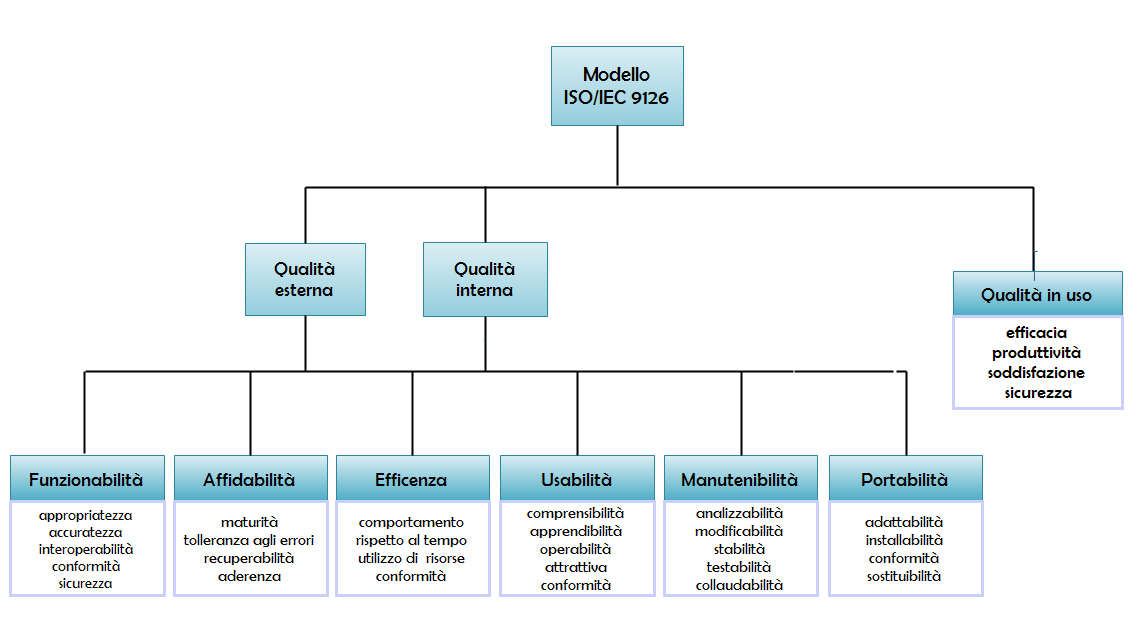
\includegraphics[width=0.7\textwidth]{./images/ISO-IEC_9126}
  \caption{Rappresentazione del modello ISO/IEC 9126:2001}
  \label{fig:ISO-IEC_9126}
\end{figure}


\subsubsection{Funzionalità}
È un Requisito\ped{g} funzionale che indica la capacità del Software\ped{g} di soddisfare le esigenze esposte dal capitolato ed individuate durante l’analisi dei Requisiti\ped{g}. Per valutare questa caratteristica si considerano l'appropriatezza e l'accuratezza delle funzioni\ped{g} offerte, l'interoperabilità del prodotto rispetto ai diversi sistemi e la sicurezza offerta per la protezione dei dati.\\ 
\textbf{Quantificazione del raggiungimento dell’obbiettivo di qualità:} la misurazione
del raggiungimento di questo obiettivo si calcolerà verificando la quantità
di Requisiti\ped{g} soddisfatti che avranno un riscontro in elementi\ped{g} funzionanti
nell’applicazione prodotta. La soglia di sufficienza sarà quindi data dal soddisfacimento
di tutti i Requisiti\ped{g} obbligatori previsti dal capitolato d’appalto.

\subsubsection{Affidabilità}
È un Requisito\ped{g} non funzionale che indica la capacità del Software\ped{g} di svolgere correttamente il suo compito, mantenendo delle buone prestazioni anche al variare dell'ambiente nel tempo; vengono considerate la sua tolleranza agli errori, la capacità di evitare fallimenti nell’esecuzione a seguito di malfunzionamenti (detta maturità) e la recuperabilità dei dati e delle prestazioni nell'eventualità di un malfunzionamento inevitabile.\\ \textbf{Quantificazione del raggiungimento dell’obbiettivo di qualità:} la misurazione del raggiungimento di questo obiettivo si calcolerà confrontando il numero di esecuzioni totale con quelle andate a buon fine e che hanno mantenuto un livello di prestazioni tali da poter permettere l’utilizzo previsto del prodotto

\subsubsection{Efficienza}
È un Requisito\ped{g} non funzionale che indica il rapporto tra le prestazioni e le Risorse\ped{g} disponibili.
Si valuta se il Software\ped{g} utilizza al meglio le Risorse\ped{g} a sua disposizione per fornire le funzionalità richieste, considerando il suo comportamento rispetto al tempo, ossia la velocità di risposta e d'elaborazione in determinate condizioni, che rispetto all’uso delle Risorse\ped{g}, data dalla capacità d'utilizzarne una quantità adeguata ad eseguire le funzioni\ped{g} richieste. \\
\textbf{Quantificazione del raggiungimento dell’obbiettivo di qualità:} Un modo per valutare l’efficienza di un Software\ped{g} è calcolarne i tempi di attesa in seguito all’esecuzione di un comando, tuttavia, nel caso del prodotto Premi l'efficienza è limitata anche dallo stato della rete e dall'utilizzo di componenti grafiche quali video o immagini; per questo motivo il gruppo non può garantire tempi di risposta brevi per ogni azione compiuta dall’utente, ma si impegna a non appesantire ulteriormente tali componenti.

\subsubsection{Usabilità}
È un Requisito\ped{g} non funzionale che indica la capacità del Software\ped{g} di essere compreso, appreso ed usato con soddisfazione dall'utente. \\
Per far ciò il prodotto deve soddisfare condizioni di comprensibilità, apprendibilità ed operabilità; deve inoltre avere una certa attrattiva nei confronti dell'utente allo scopo di rendergliene piacevole l’utilizzo.\\ \textbf{Quantificazione del raggiungimento dell’obbiettivo di qualità:} Questa caratteristica non è facilmente misurabile in quanto non esistono metriche\ped{g} per quantificarla, perciò si farà affidamento alle linee guida del material design\ped{g} fornite da Google, dato l'alto tasso di adozione rispetto ad altre linee guida.

\subsubsection{Manutenibilità}
È un Requisito\ped{g} non funzionale che indica la capacità del Software\ped{g} di essere corretto, migliorato o adattato con impegno contenuto; a tale scopo esso deve essere facilmente analizzabile e modificabile, deve garantire stabilità a seguito di modifiche e la testabilità di tali modifiche.  \\
\textbf{Quantificazione del raggiungimento dell’obbiettivo di qualità:} Per la misurazione di questo Requisito\ped{g} si fa riferimento alle metriche\ped{g} descritte nella sezione \ref{sec:metriche}.

\subsubsection{Portabilità}
È un Requisito\ped{g} non funzionale che indica la capacità del Software\ped{g} di adattarsi al cambio di dispositivo e sistema operativo, limitando la necessità di apportare cambiamenti.\\
\textbf{Quantificazione del raggiungimento dell’obbiettivo di qualità:} Per soddisfare questa caratteristica, come espresso dal capitolato, è necessario che il Software\ped{g} funzioni\ped{g} sia su computer (indipendentemente dal loro sistema operativo) e su dispositivi mobile\ped{g} Android\ped{g}, iOS e Windows\ped{g} Phone.

\subsection{Procedure di controllo di qualità di processo}
Per applicare il modello SPICE\ped{g} si utilizzerà il ciclo di Deming. Il ciclo di Deming è un sistema iterativo per il miglioramento continuo della qualità dei Processi\ped{g} e dei prodotti da essi risultanti, che permette di riconoscere lo stato di avanzamento di un Progetto\ped{g} fornendo un metodo di lavoro logico e sistematico.

\begin{figure}[h]
  \centering
    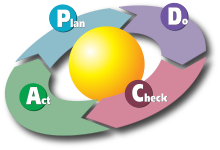
\includegraphics[width=0.5\textwidth]{./images/deming}
  \caption{Schema PDCA}
  \label{fig:deming}
\end{figure}

È chiamato anche ciclo PDCA, in quanto è definito dall'Iterazione\ped{g} delle quattro fasi:
 
\begin{itemize}
\item \textbf{Plan}: si stabiliscono obiettivi e Processi\ped{g} necessari ad ottenere risultati conformi agli obiettivi attesi;
\item \textbf{Do}: si implementa il piano, si esegue il Processo\ped{g} e si realizza il prodotto. Si raccolgono dati da analizzare nei passi successivi;
\item \textbf{Check}: si studiano i risultati ottenuti tramite la raccolta dei dati nella fase "Do" e si paragonano con i risultati attesi (gli obiettivi stabiliti nella fase "Plan"), per verificare la presenza di incongruenze. Si evidenziano le differenze nell'implementazione rispetto al piano;
\item \textbf{Act}: se la fase di Check evidenzia che gli obiettivi fissati nel Plan e implementati nel Do rappresentano un miglioramento rispetto alla baseline precedente, si stabilisce una nuova baseline; in caso contrario la baseline non cambia. In entrambi i casi se la fase di Check ha evidenziato differenze rispetto alle aspettative, sarà necessario svolgere nuovamente il ciclo di PDCA.
\end{itemize}
Una descrizione di come il gruppo applicherà il PDCA è riportata nelle \NormeDiProgetto (\S5.1).